\section{User Account Control (UAC)}


\label{windows_knowledge:fundamentals:security:uac}

\href{https://docs.microsoft.com/en-us/windows/security/identity-protection/user-account-control/how-user-account-control-works}{User
Account Control (UAC)}~\ref{windows_knowledge:ad:rights_privileges:uac}
 is a Windows security feature that forces any new process to run in the
 security context of a non-privileged account by default. This policy applies
 to processes started by any user, including administrators themselves. The
 idea is that we can't solely rely on the user's identity to determine if some
 actions should be authorized.

 \subsection{UAC elevation}
Each app that requires the administrator access token must prompt for consent.
The one exception is the relationship that exists between parent and child
processes. Child processes inherit the user's access token from the parent
process. Both the parent and child processes, however, must have the same
integrity level.

When a standard user attempts to run an app that requires an administrator
access token, UAC requires that the user provide valid administrator
credentials.

 \subsection{Mandatory Integrity Controls and Integrity level}
\href{https://docs.microsoft.com/en-us/windows/win32/secauthz/mandatory-integrity-control}{Mandatory
Integrity Control (MIC)} provides a mechanism for controlling access to
securable objects. This mechanism is in addition to discretionary access
control and evaluates access before access checks against an object's
discretionary access control list (DACL) are evaluated. 

MIC uses \emph{integrity levels} and mandatory policy to evaluate access. Security
principals and securable objects are assigned integrity levels that determine
their levels of protection or access. In general terms, users or processes with
a higher IL access token will be able to access resources with lower or equal
ILs.

The following 4 ILs are used by Windows, ordered from lowest to highest:
\begin{tabularx}{\linewidth}{|l|X|}
    \hline
Integrity Level	& Use \\
    \hline
Low	& Generally used for interaction with the Internet (i.e. Internet
Explorer). Has very limited permissions. \\
    \hline
Medium &	Assigned to standard users and Administrators' filtered tokens.\\
    \hline
High&	Used by Administrators' elevated tokens if UAC is enabled. If UAC is
disabled, all administrators will always use a high IL token. \\
    \hline
System &	Reserved for system use.\\
    \hline
\end{tabularx}

When a process requires to access a resource, it will inherit the calling user's access token and its associated IL. The same occurs if a process forks a child.

Regarding tokens:
\begin{itemize}
    \item token of a non-administrator has a medium IL
    \item Filtered token~\ref{win:filtered-token} of an Administrator has a
        medium IL
    \item Elevated token of an Administrator has a high IL
\end{itemize}

\subsection{UAC settings}
UAC can be configured to run at four different notification levels:
\begin{itemize}
    \item {\bf Always notify}: Notify and prompt the user for authorization
        when making changes to Windows settings or when a program tries to
        install applications or make changes to the computer.
    \item {\bf Notify me only when programs try to make changes to my
            computer}: Notify and prompt the user for authorization when a
            program tries to install applications or make changes to the
            computer. Administrators won't be prompted when changing Windows
            settings.
    \item {\bf Notify me only when programs try to make changes to my computer
        (do not dim my desktop)}: Same as above, but won't run the UAC prompt
        on a secure desktop.
    \item {\bf Never notify}: Disable UAC prompt. Administrators will run everything using a high privilege token.
\end{itemize}

By default, UAC is configured on the Notify me only when programs try to make
changes to my computer level.

From an attacker's perspective, the three lower security levels are equivalent,
and only the Always notify setting presents a difference.
\subsubsection{Security policy settings}
See
\href{https://docs.microsoft.com/en-us/windows/security/identity-protection/user-account-control/user-account-control-security-policy-settings}{Microsoft
 documentation} for more information.

\subsubsection{Group Policy settings}
See \href{https://docs.microsoft.com/en-us/windows/security/identity-protection/user-account-control/user-account-control-group-policy-and-registry-key-settings#group-policy-settings}{Microsoft
 documentation} for more information.

\subsubsection{Registry key settings}

 The parameters responsible for the behavior of User Account Control are
 located under the registry key 
 \begin{verbatim}
 HKLM\SOFTWARE\Microsoft\Windows\CurrentVersion\Policies\System
 \end{verbatim}

 See
 \href{https://docs.microsoft.com/en-us/windows/security/identity-protection/user-account-control/user-account-control-group-policy-and-registry-key-settings#registry-key-settings}{Microsoft
 documentation} for more information.

\subsection{Application Information Service}
At the heart of UAC, there is the Application Information Service or Appinfo. Whenever a user requires elevation, the following occurs:
\begin{enumerate}
        \item The user requests to run an application as administrator.
        \item A ShellExecute API call is made using the runas verb.
        \item The request gets forwarded to Appinfo to handle elevation.
        \item The application manifest is checked to see if AutoElevation is allowed (more on this later).
        \item Appinfo executes consent.exe, which shows the UAC prompt on a secure desktop. A secure desktop is simply a separate desktop that isolates processes from whatever is running in the actual user's desktop to avoid other processes from tampering with the UAC prompt in any way.
        \item If the user gives consent to run the application as administrator, the Appinfo service will execute the request using a user's Elevated Token. Appinfo will then set the parent process ID of the new process to point to the shell from which elevation was requested.
\end{enumerate}

    The following diagram, adapted from the source here, illustrates how UAC works.

\begin{figure}
  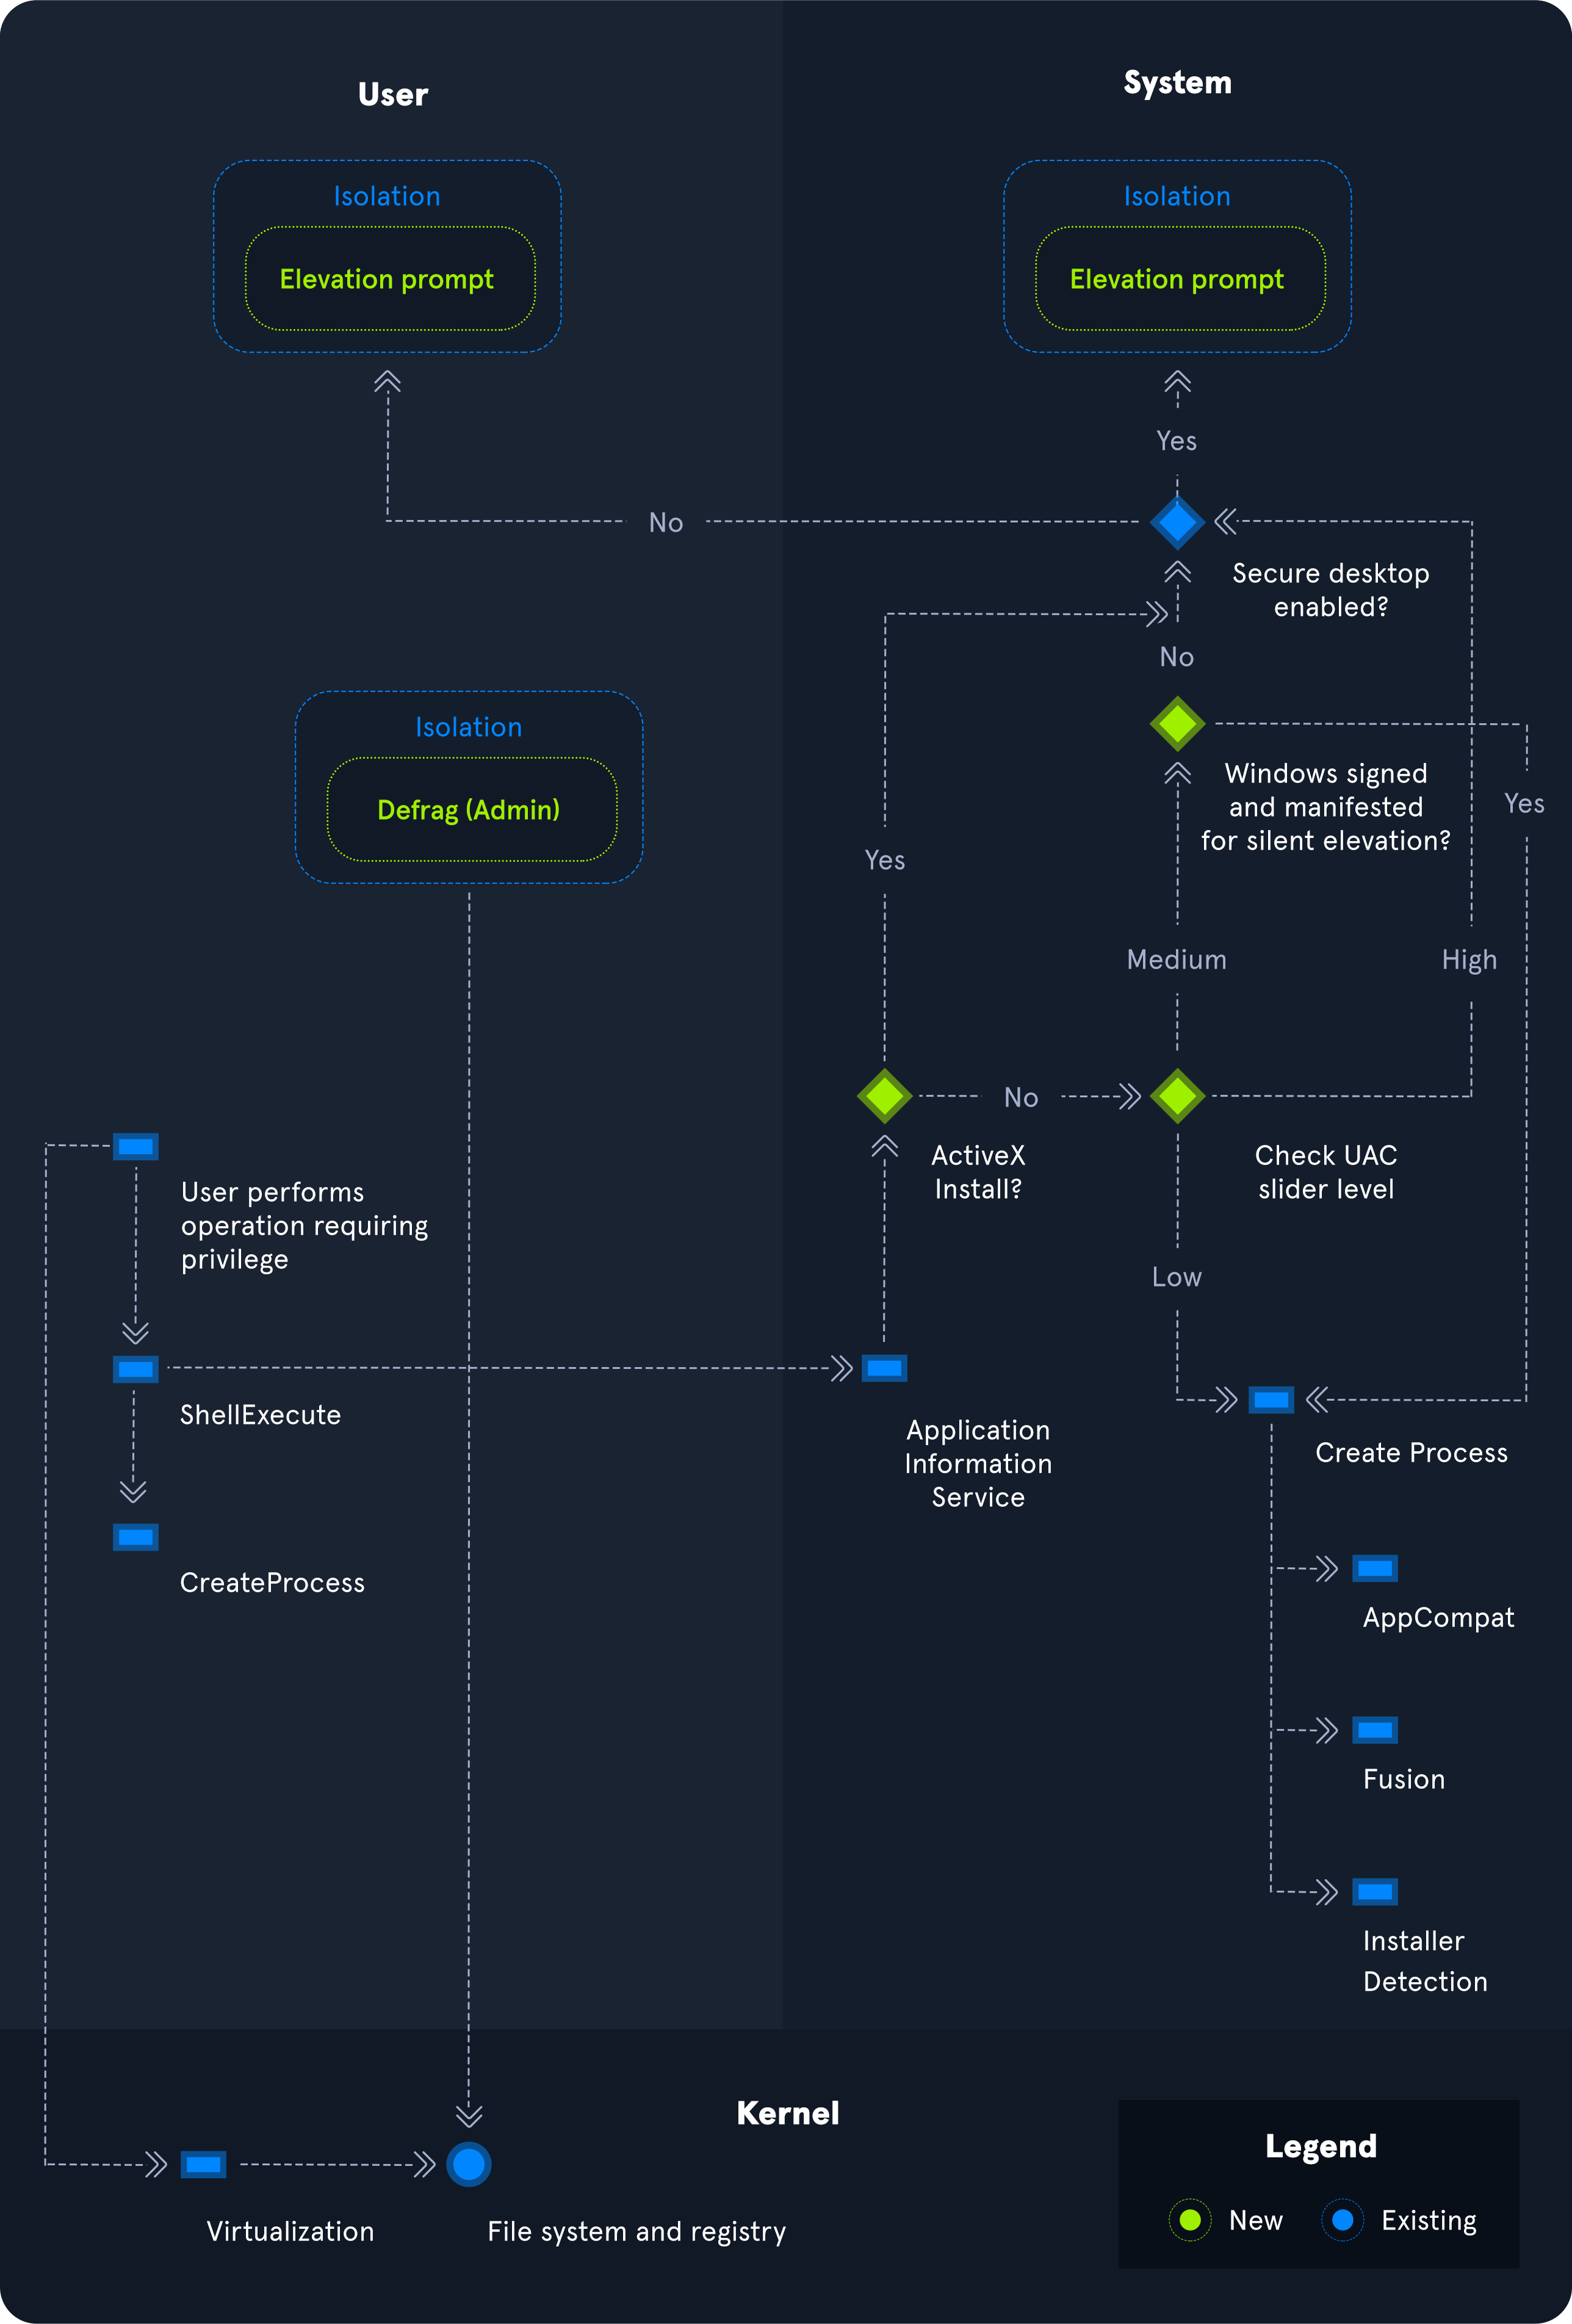
\includegraphics[width=\linewidth]{windows_knowledge/security/images/uac_architecture.png}
  \caption{UAC architecture}
  \label{fig:uac-architecture}
\end{figure}


\subsection{Auto-elevating processes}

Some programs are autoelevated automatically if the user belongs to the
administrator group. 

To bypass the UAC (elevate from medium integrity level to high) some
attackers use this kind of binaries to execute arbitrary code because it will
be executed from a High level integrity process.


For an application, some requirements need to be met to
auto-elevate:
\begin{itemize}
    \item The binary has to be signed by Microsoft Publisher 
    \item the binary must be contained in a trusted directory (like \verb+%SystemRoot%/System32/+ or
    \verb+%ProgramFiles%/+)
\end{itemize}

Depending on the type of application, additional requirements may apply:

\begin{itemize}
    \item Executable files (.exe) must declare the autoElevate element inside
        their manifests.  \verb+sigcheck.exey+ from Sysinternals allow to check
        the Manifest of a binary.

    \item mmc.exe will auto elevate depending on the .msc snap-in that the user requests. Most of the .msc files included with Windows will auto elevate.
    \item Windows keeps an additional list of executables that auto elevate even when not requested in the manifest. This list includes pkgmgr.exe and spinstall.exe, for example.
    \item COM objects can also request auto-elevation by configuring some
        registry keys (See
        \href{https://docs.microsoft.com/en-us/windows/win32/com/the-com-elevation-moniker}{Windows
    documentation}).
\end{itemize}


